\documentclass[landscape,final,paperwidth=75in,paperheight=48in,fontscale=0.285]{baposter}
%\usepackage{calc,array} 
\usepackage{graphicx} % Required for including images
\usepackage{amsmath}  % For typesetting math
\usepackage{amssymb}  % Adds new symbols to be used in math mode
\usepackage{relsize}  % Change size of text /smaller, /larger
\usepackage{multirow} % Allows table cells to span more than one row of the table
\usepackage{rotating} % Rotate figures and tables
\usepackage{bm}       % Allows a math expression to be bold
\usepackage{url}      % Allows email address and websites
\usepackage{gensymb}  % Allows degree symbol

\usepackage{float}
\usepackage{caption} % Required for specifying captions to tables and figures
\usepackage{wrapfig} % Wrap text around figure
\usepackage[export]{adjustbox}

%\captionsetup[figure]{font=Large,skip=0pt,labelformat=empty,justification=raggedright,singlelinecheck=false}

\usepackage{multicol} % Required for multiple columns

\newcommand{\BIBdecl}{\setlength{\itemsep}{-0.25 em}} %Removes line space between references

% Fonts
%\usepackage{times}
%\usepackage{helvet}
%\usepackage{bookman}
\usepackage{palatino}

%\newcommand{\captionfont}{\footnotesize}

\graphicspath{{images/}{../images/}}
%\usetikzlibrary{calc}

\newcommand{\SET}[1]  {\ensuremath{\mathcal{#1}}}
\newcommand{\MAT}[1]  {\ensuremath{\boldsymbol{#1}}}
\newcommand{\VEC}[1]  {\ensuremath{\boldsymbol{#1}}}
\newcommand{\Video}{\SET{V}}
\newcommand{\video}{\VEC{f}}
\newcommand{\track}{x}
\newcommand{\Track}{\SET T}
\newcommand{\LMs}{\SET L}
\newcommand{\lm}{l}
\newcommand{\PosE}{\SET P}
\newcommand{\posE}{\VEC p}
\newcommand{\negE}{\VEC n}
\newcommand{\NegE}{\SET N}
\newcommand{\Occluded}{\SET O}
\newcommand{\occluded}{o}

%%%%%%%%%%%%%%%%%%%%%%%%%%%%%%%%%%%%%%%%%%%%%%%%%%%%%%%%%%%%%%%%%%%%%%%%%%%%%%%%
% Multicol Settings
%%%%%%%%%%%%%%%%%%%%%%%%%%%%%%%%%%%%%%%%%%%%%%%%%%%%%%%%%%%%%%%%%%%%%%%%%%%%%%%%
\setlength{\columnsep}{1.5em}
\setlength{\columnseprule}{0mm}
%%%%%%%%%%%%%%%%%%%%%%%%%%%%%%%%%%%%%%%%%%%%%%%%%%%%%%%%%%%%%%%%%%%%%%%%%%%%%%%%
% Save space in lists. Use this after the opening of the list
%%%%%%%%%%%%%%%%%%%%%%%%%%%%%%%%%%%%%%%%%%%%%%%%%%%%%%%%%%%%%%%%%%%%%%%%%%%%%%%%
\newcommand{\compresslist}{%
\setlength{\itemsep}{1pt}%
\setlength{\parskip}{0pt}%
\setlength{\parsep}{0pt}%
}
%%%%%%%%%%%%%%%%%%%%%%%%%%%%%%%%%%%%%%%%%%%%%%%%%%%%%%%%%%%%%%%%%%%%%%%%%%%%%%
%%% Begin of Document
%%%%%%%%%%%%%%%%%%%%%%%%%%%%%%%%%%%%%%%%%%%%%%%%%%%%%%%%%%%%%%%%%%%%%%%%%%%%%%

\begin{document}

%%%%%%%%%%%%%%%%%%%%%%%%%%%%%%%%%%%%%%%%%%%%%%%%%%%%%%%%%%%%%%%%%%%%%%%%%%%%%%
%%% Here starts the poster
%%%---------------------------------------------------------------------------
%%% Format it to your taste with the options
%%%%%%%%%%%%%%%%%%%%%%%%%%%%%%%%%%%%%%%%%%%%%%%%%%%%%%%%%%%%%%%%%%%%%%%%%%%%%%
% Define some colors

%\definecolor{lightblue}{cmyk}{0.83,0.24,0,0.12}
\definecolor{lightblue}{rgb}{0.145,0.6666,1}

%\newtcolorbox{demobox}[1][]{colback=white,colframe=lightblue,width=0.33\linewidth,nobeforeafter,box align=top,before=\noindent,#1}

%%
\begin{poster}%
  % Poster Options
  {
  % Show grid to help with alignment
  grid=false,
  % Column spacing
  colspacing=.6em,      % default = 1em
  % Color style
  bgColorOne=white,
  bgColorTwo=white,
  borderColor=lightblue,
  headerColorOne=black,
  headerColorTwo=lightblue,
  headerFontColor=white,
  boxColorOne=white,
  boxColorTwo=lightblue,
  % Format of textbox
  textborder=roundedleft,
  % Format of text header
  eyecatcher=true,          % true when you want a logo on the left side of the title otherwise false
  headerborder=closed,
  headerheight=0.07\textheight, % default = .1/textheight
  columns=4, %default=4 for landscape posters maximum columns=6
%  textfont=\sc, An example of changing the text font
  headershape=roundedright,
  headershade=shadelr,
  headerfont=\Large\bf\textsc, %Sans Serif
  textfont={\setlength{\parindent}{1.5em}},
  boxshade=plain,
%  background=shade-tb,
  background=plain,
  linewidth=2pt
  }
  % Left Header image (shows up when eyecatcher=true)
  % University Logo
  {
  
\includegraphics[height=3em]{img/databrary.png}
  }
  % Title
  {
  \vspace{-0.2ex}
  \bf{Sharing nicely with others: Moving developmental scientists toward open data sharing}
  \vspace{0.1ex}
  }
  % Authors
  {
  Rick O. Gilmore \emph{(rick.gilmore@databrary.org)}\textsuperscript{1,2}, Karen Adolph \emph{(kea1@nyu.edu)}\textsuperscript{1,3}, Andrea R. Seisler \emph{(andrea.seisler@databrary.org)}\textsuperscript{1,2} \\
  \smaller \textsuperscript{1}Databrary, \textsuperscript{2}Penn State University, \textsuperscript{3}New York University \\
  }
  % Right Header Image
 {
 
\includegraphics[height=3em]{img/datavyu.png}
 % datavyu logo or DEVSEC 2018
 }

%%%%%%%%%%%%%%%%%%%%%%%%%%%%%%%%%%%%%%%%%%%%%%%%%%%%%%%%%%%%%%%%%%%%%%%%%%%%%%
%%% Now define the boxes that make up the poster
%%%---------------------------------------------------------------------------
%%% Each box has a name and can be placed absolutely or relatively.
%%% The only inconvenience is that you can only specify a relative position
%%% towards an already declared box. So if you have a box attached to the
%%% bottom, one to the top and a third one which should be in between, you
%%% have to specify the top and bottom boxes before you specify the middle
%%% box.
%%%%%%%%%%%%%%%%%%%%%%%%%%%%%%%%%%%%%%%%%%%%%%%%%%%%%%%%%%%%
%
%%%%%%%%%%%%%%%%%%%%%%%%%%%%%%%%%%%%%%%%%%%%%%%%%%%%%%%%%%%%%%%%%%%%%%%%%%%%%%
\headerbox{Abstract}{name=abstract,column=0,span = 1,row=0}
%%%%%%%%%%%%%%%%%%%%%%%%%%%%%%%%%%%%%%%%%%%%%%%%%%%%%%%%%%%%%%%%%%%%%%%%%%%%%%
{
    \par Despite an increasing push from publishers and funders toward more open scientific practices, reproducibility and transparency are hindered by the low rate at which researchers share their data and procedures. In two recent surveys, only 28.1\% of respondents (N = 83) reported sharing data with other researchers, although 50.0\% of them used an online video sharing service to view other researchers' data and 46.9\% used the same online platform to locate video clips for teaching or conference presentations. The field seems to be moving in the right direction, however, 68.8\% of the same researchers had applied for permission from their ethics board to share their data with other researchers. We discuss the challenges, and some potential solutions, to move researchers closer to open sharing of data and procedures, including: 
    \begin{enumerate}
        \item ensuring participant confidentiality and addressing privacy concerns;
        \vspace{-.5em}
        \item meeting the requirements of institutional review boards;
        \vspace{-.5em}
        \item fostering collaboration among international researchers with different institutional frameworks; and 
        \vspace{-.5em}
        \item facilitating data management and links with online repositories. 
    \end{enumerate}
    Databrary and Datavyu are among the tools that developmental scientists can use to share data and materials. Widespread sharing will accelerate discovery.   
}
%%%%%%%%%%%%%%%%%%%%%%%%%%%%%%%%%%%%%%%%%%%%%%%%%%%%%%%%%%%%%%%%%%%%%%%%%%%%%%
\headerbox{What is Databrary.org?}{name=whatDatabrary,column=0,span = 1,below=abstract}
%%%%%%%%%%%%%%%%%%%%%%%%%%%%%%%%%%%%%%%%%%%%%%%%%%%%%%%%%%%%%%%%%%%%%%%%%%%%%%
{
    Databrary.org is a web-based data library for behavioral scientists to securely store, manage, share, discover, and reuse research data, including videos, audio files, procedures and stimuli, and related metadata. 
    \vspace{-.5em}
    \begin{center}
    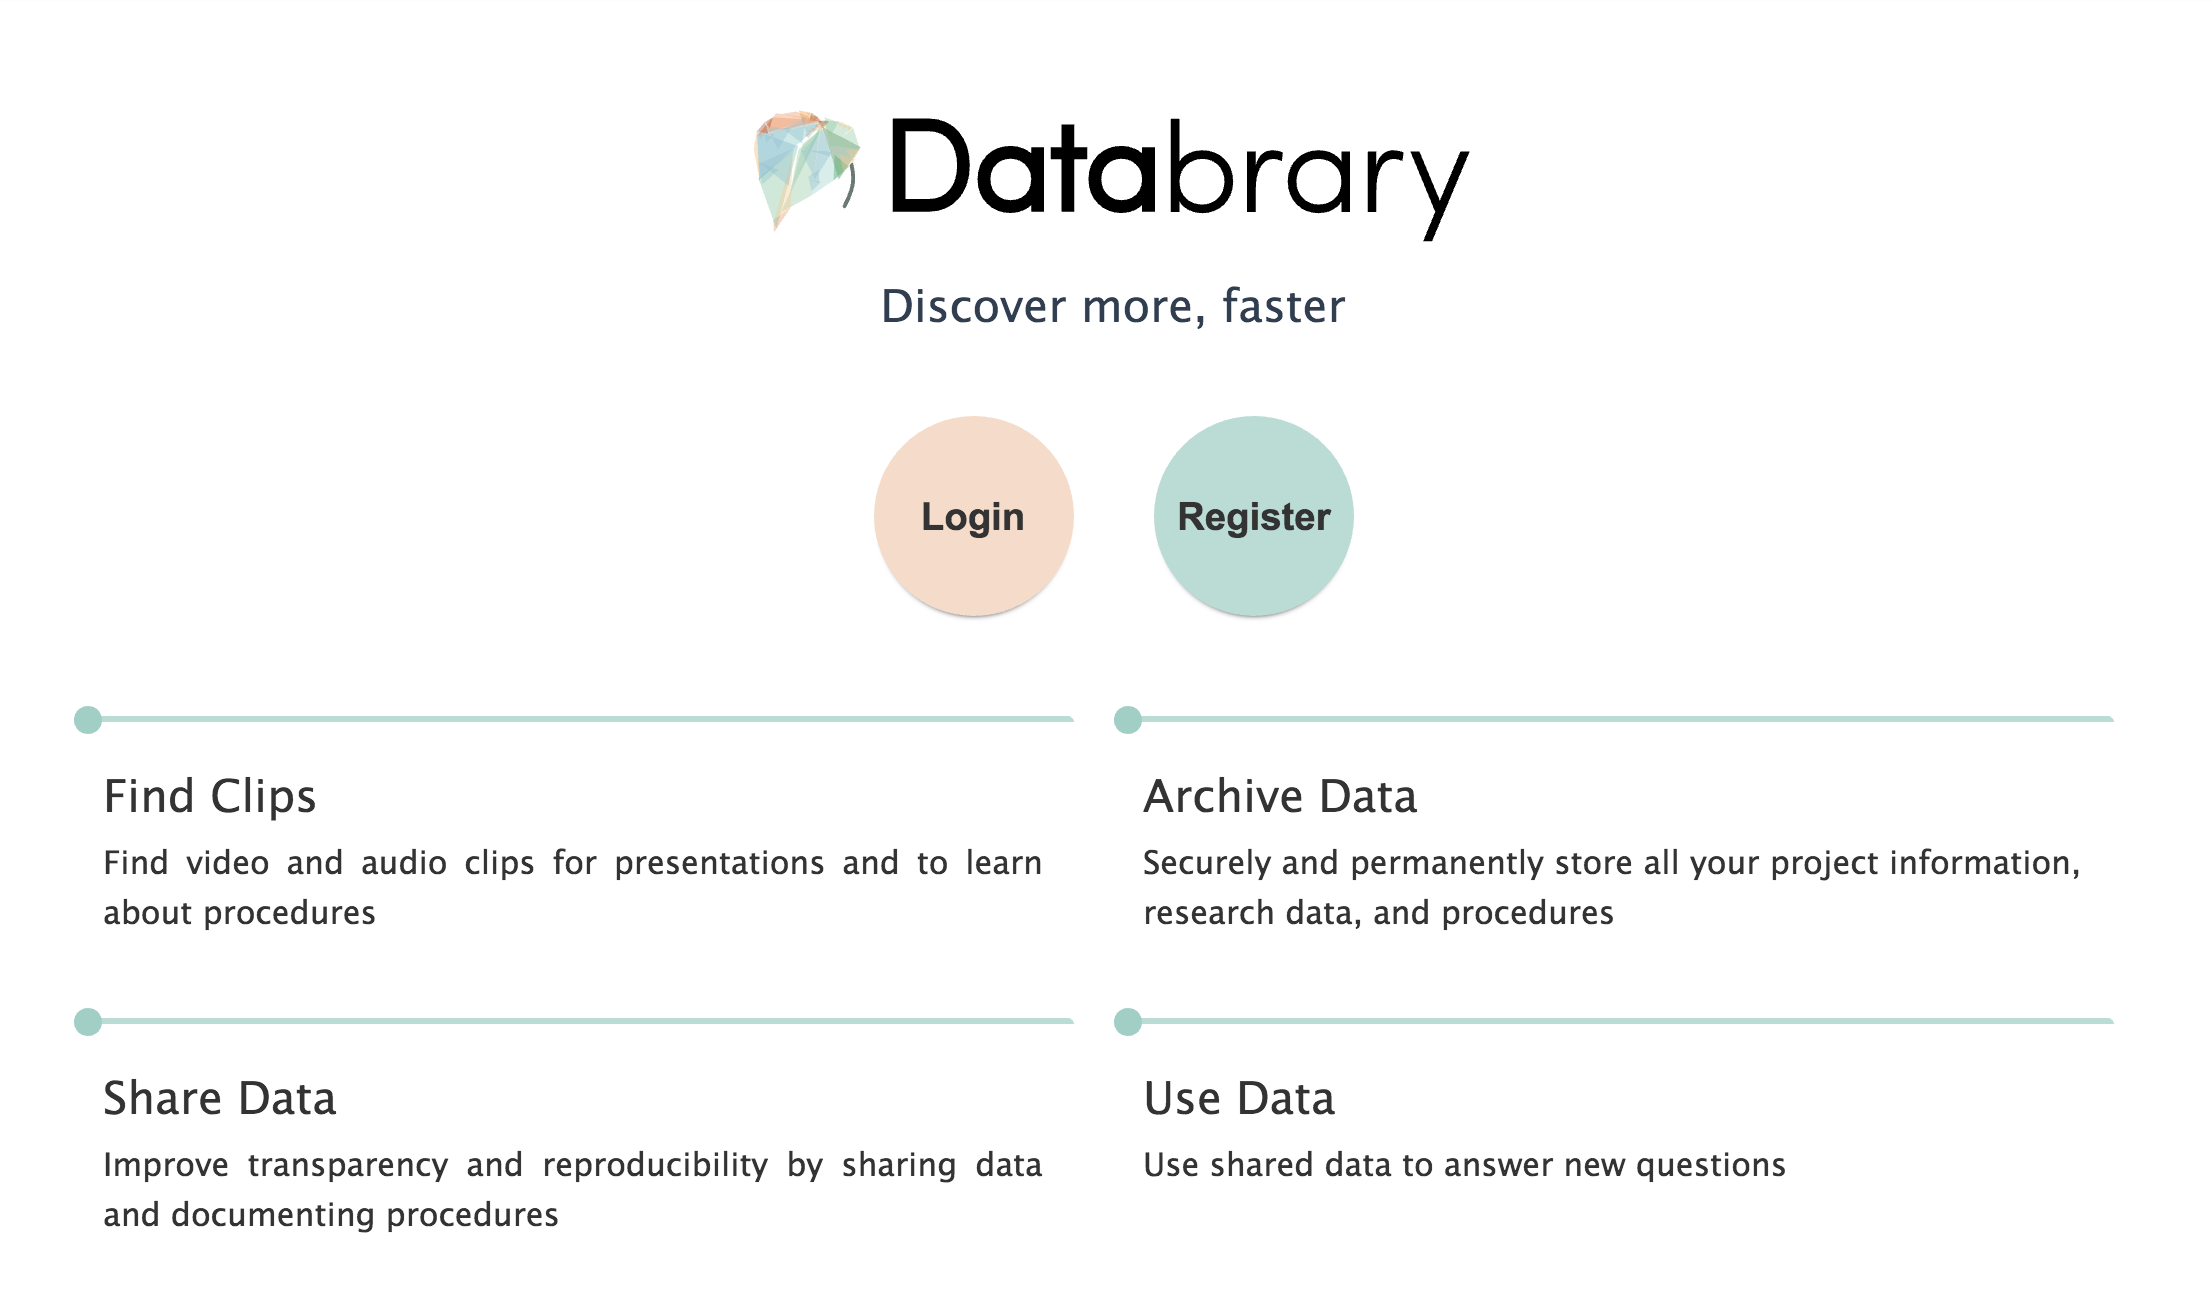
\includegraphics[scale=0.32,valign=t]{img/Databrary-DiscoverMore.png}
    \end{center}
}
%%%%%%%%%%%%%%%%%%%%%%%%%%%%%%%%%%%%%%%%%%%%%%%%%%%%%%%%%%%%%%%%%%%%%%%%%%%%%%
\headerbox{Video as Data}{name=videoData,column=1, span=3, row=0}
%%%%%%%%%%%%%%%%%%%%%%%%%%%%%%%%%%%%%%%%%%%%%%%%%%%%%%%%%%%%%%%%%%%%%%%%%%%%%%
%  volume page for shared datasets w/ investigators/collaborators from volume 8, volume 330, volume 114
%  add citation information below
{
\begin{center}
    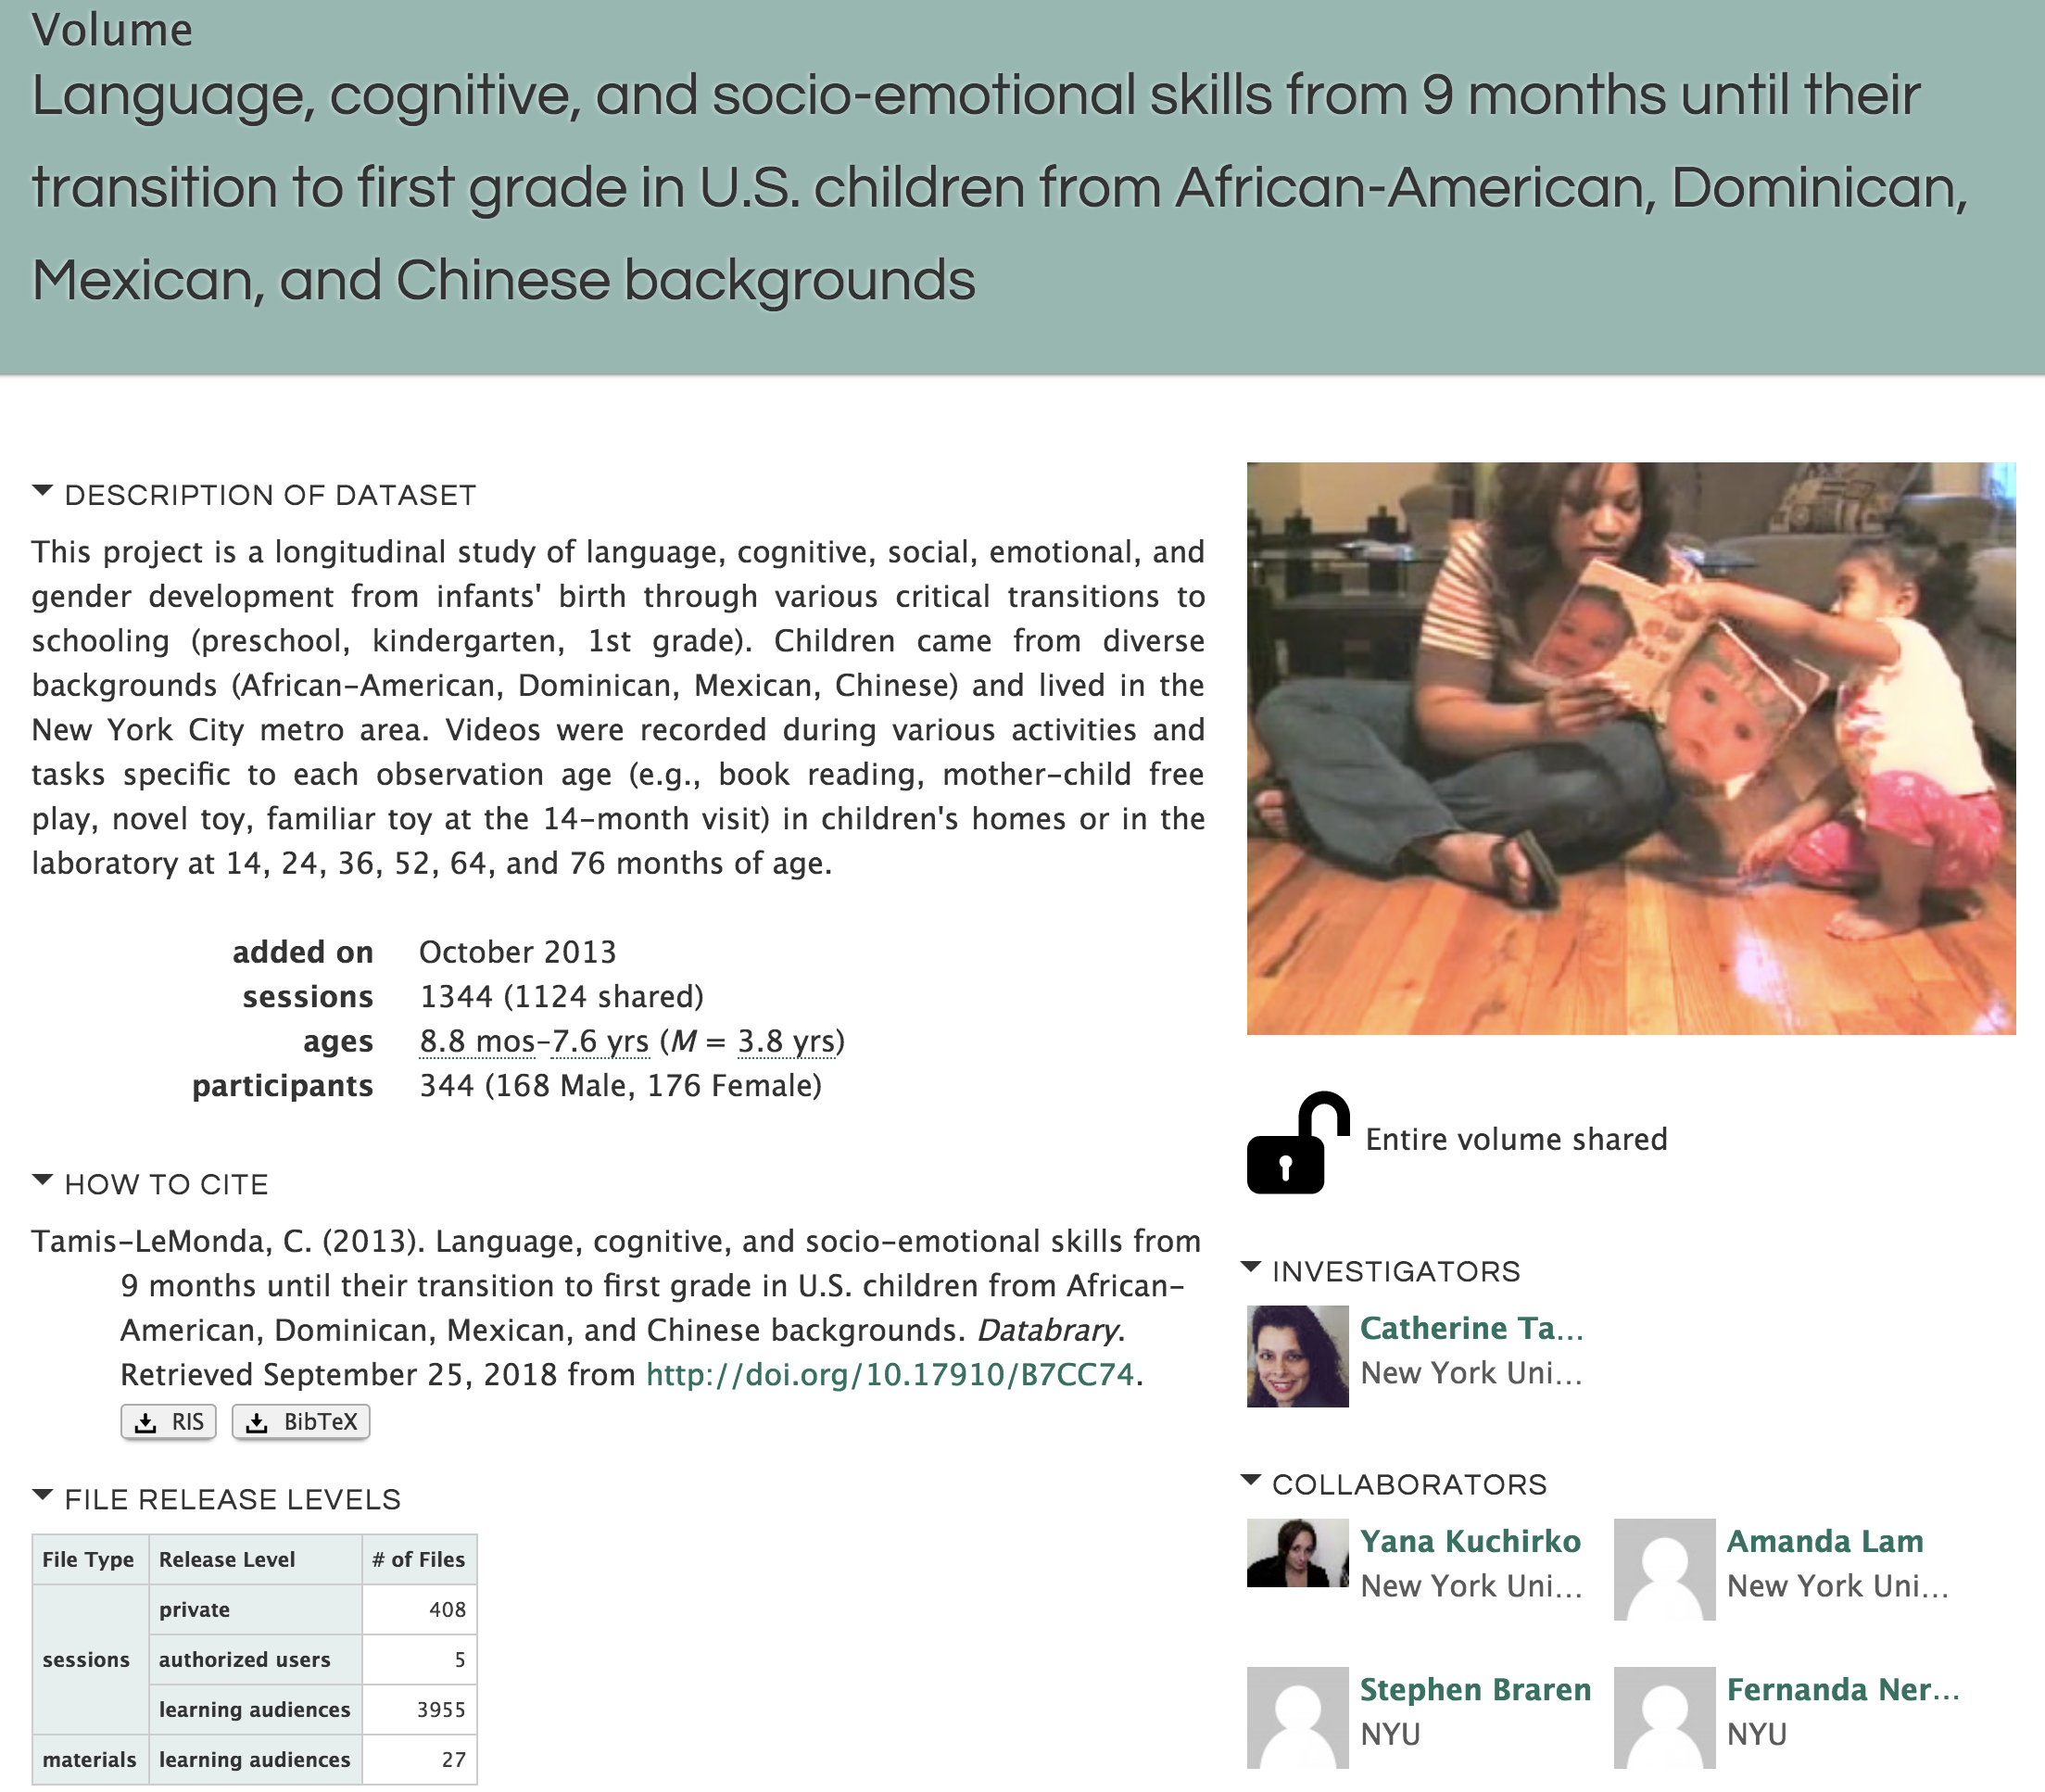
\includegraphics[scale=0.32,valign=t]{img/volume8.png}
    \hfill
    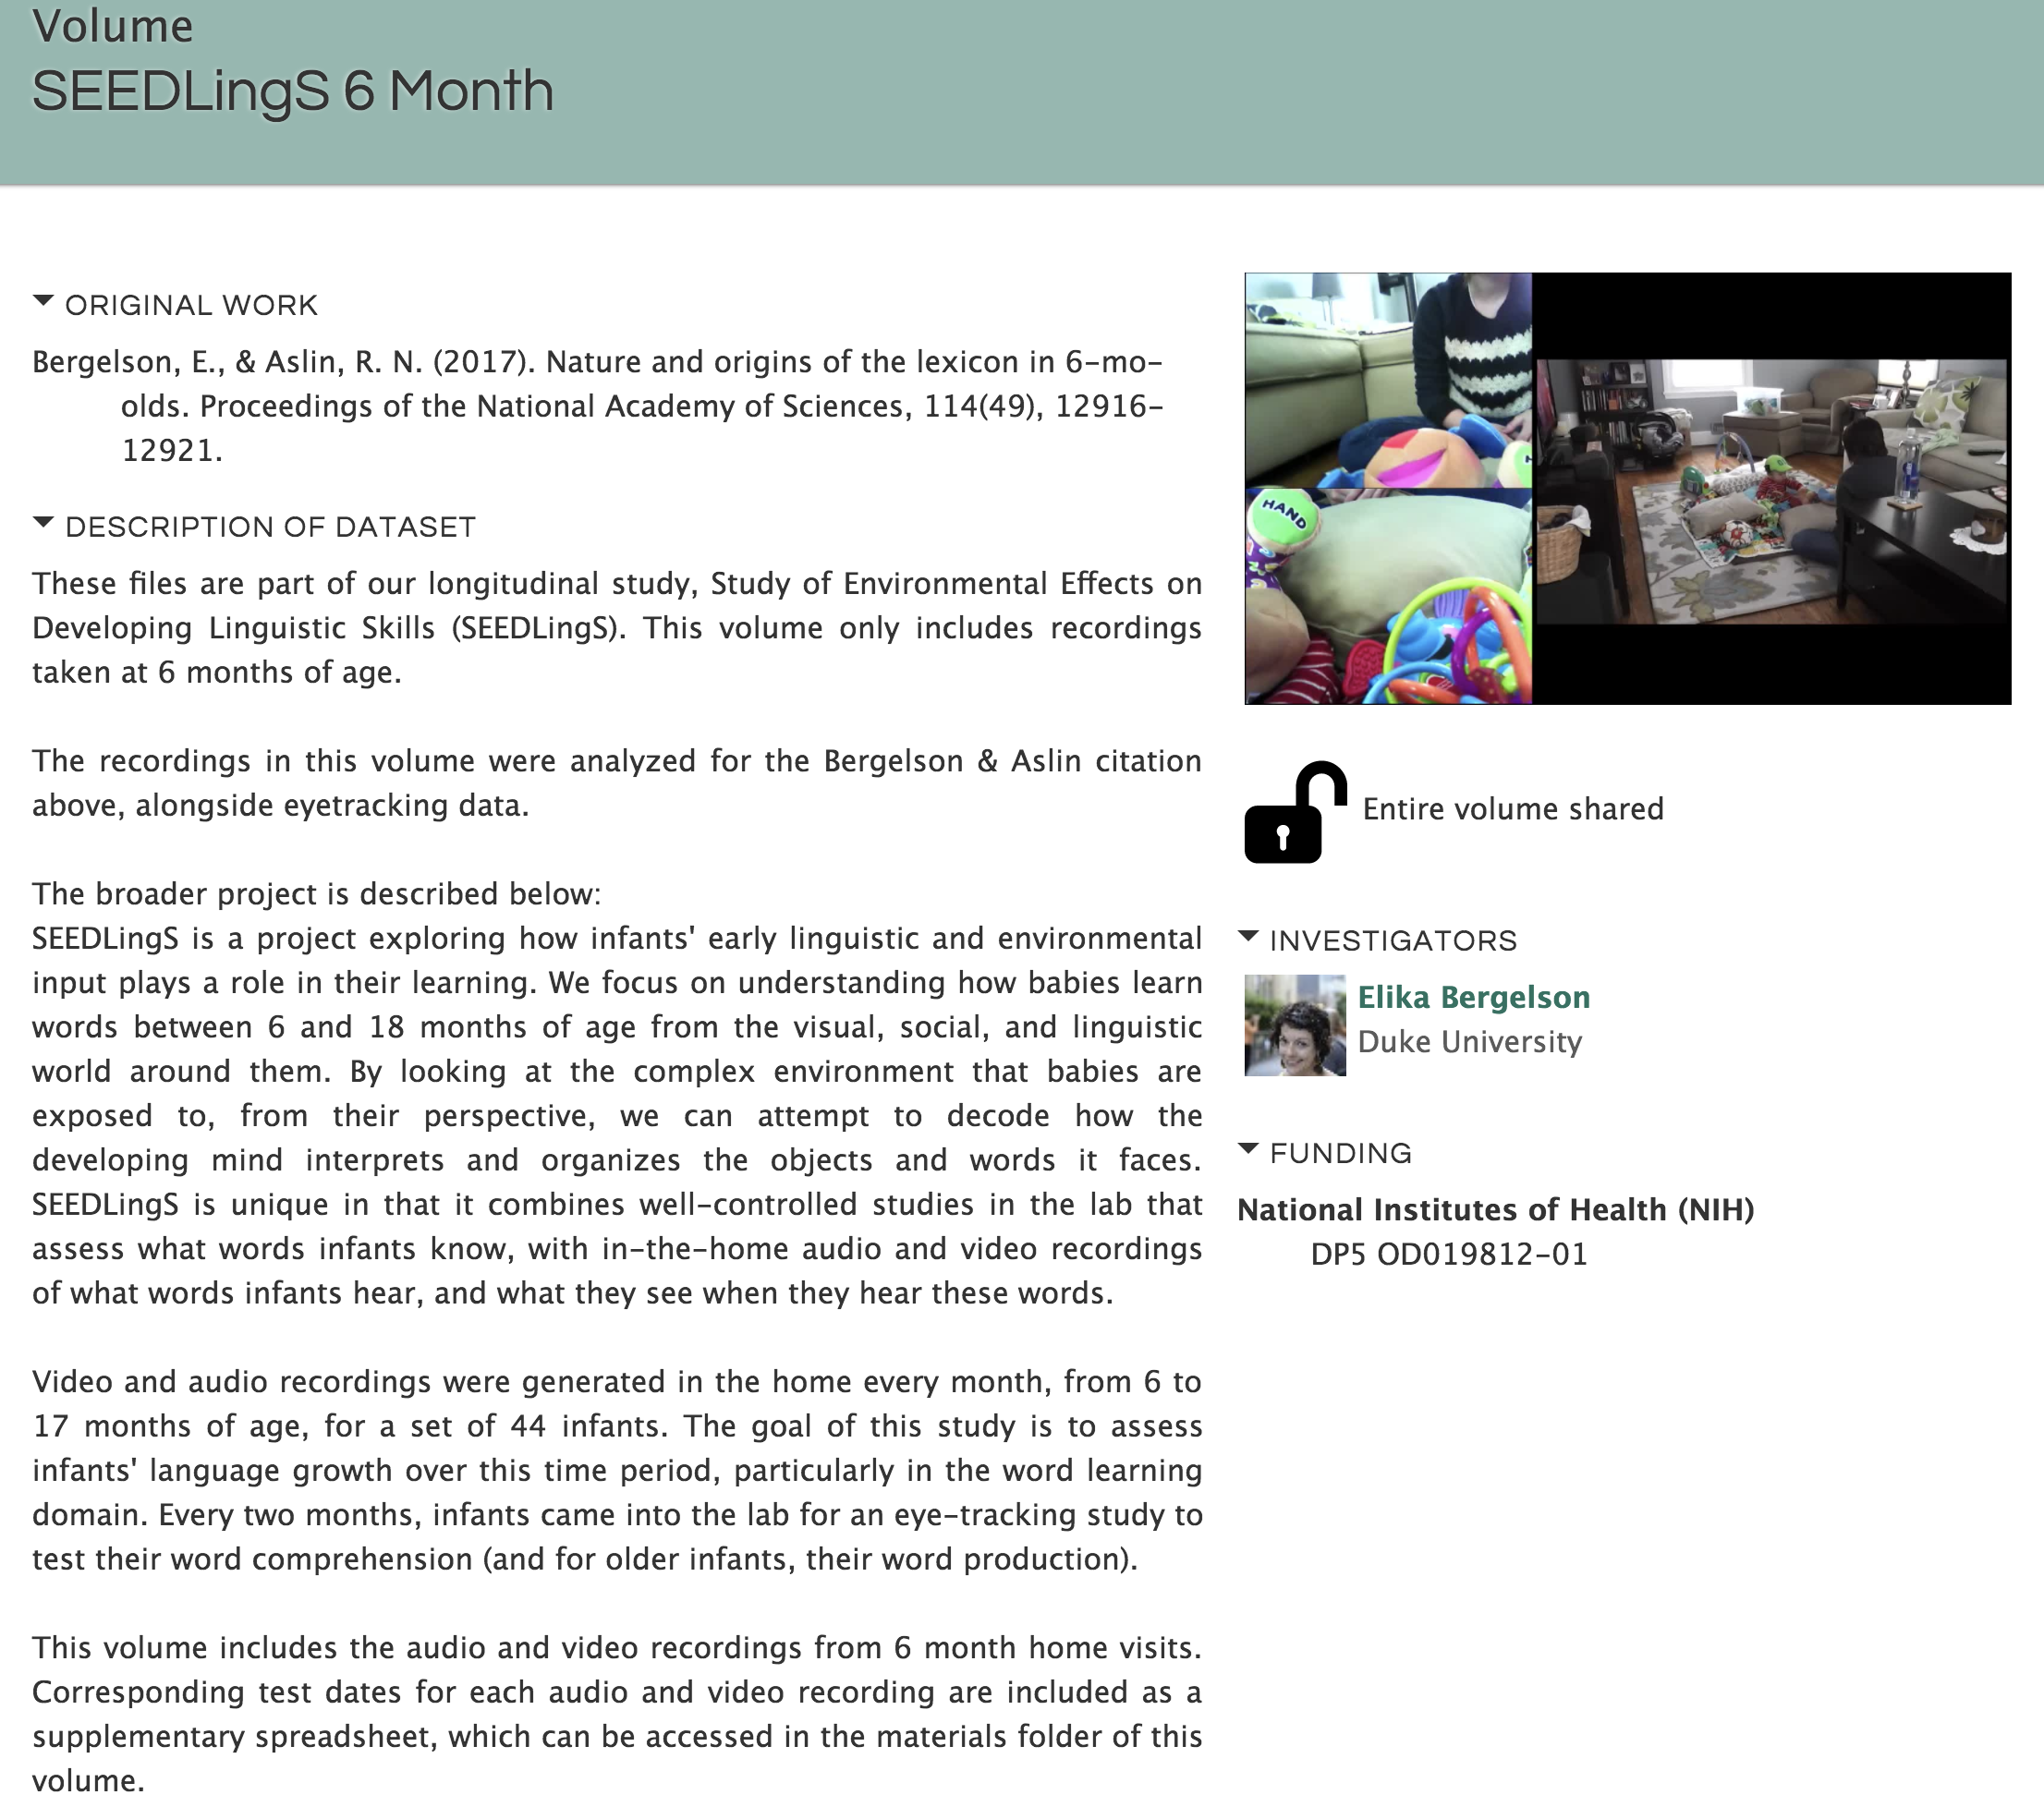
\includegraphics[scale=0.32,valign=t]{img/volume330.png}
    \hfill
    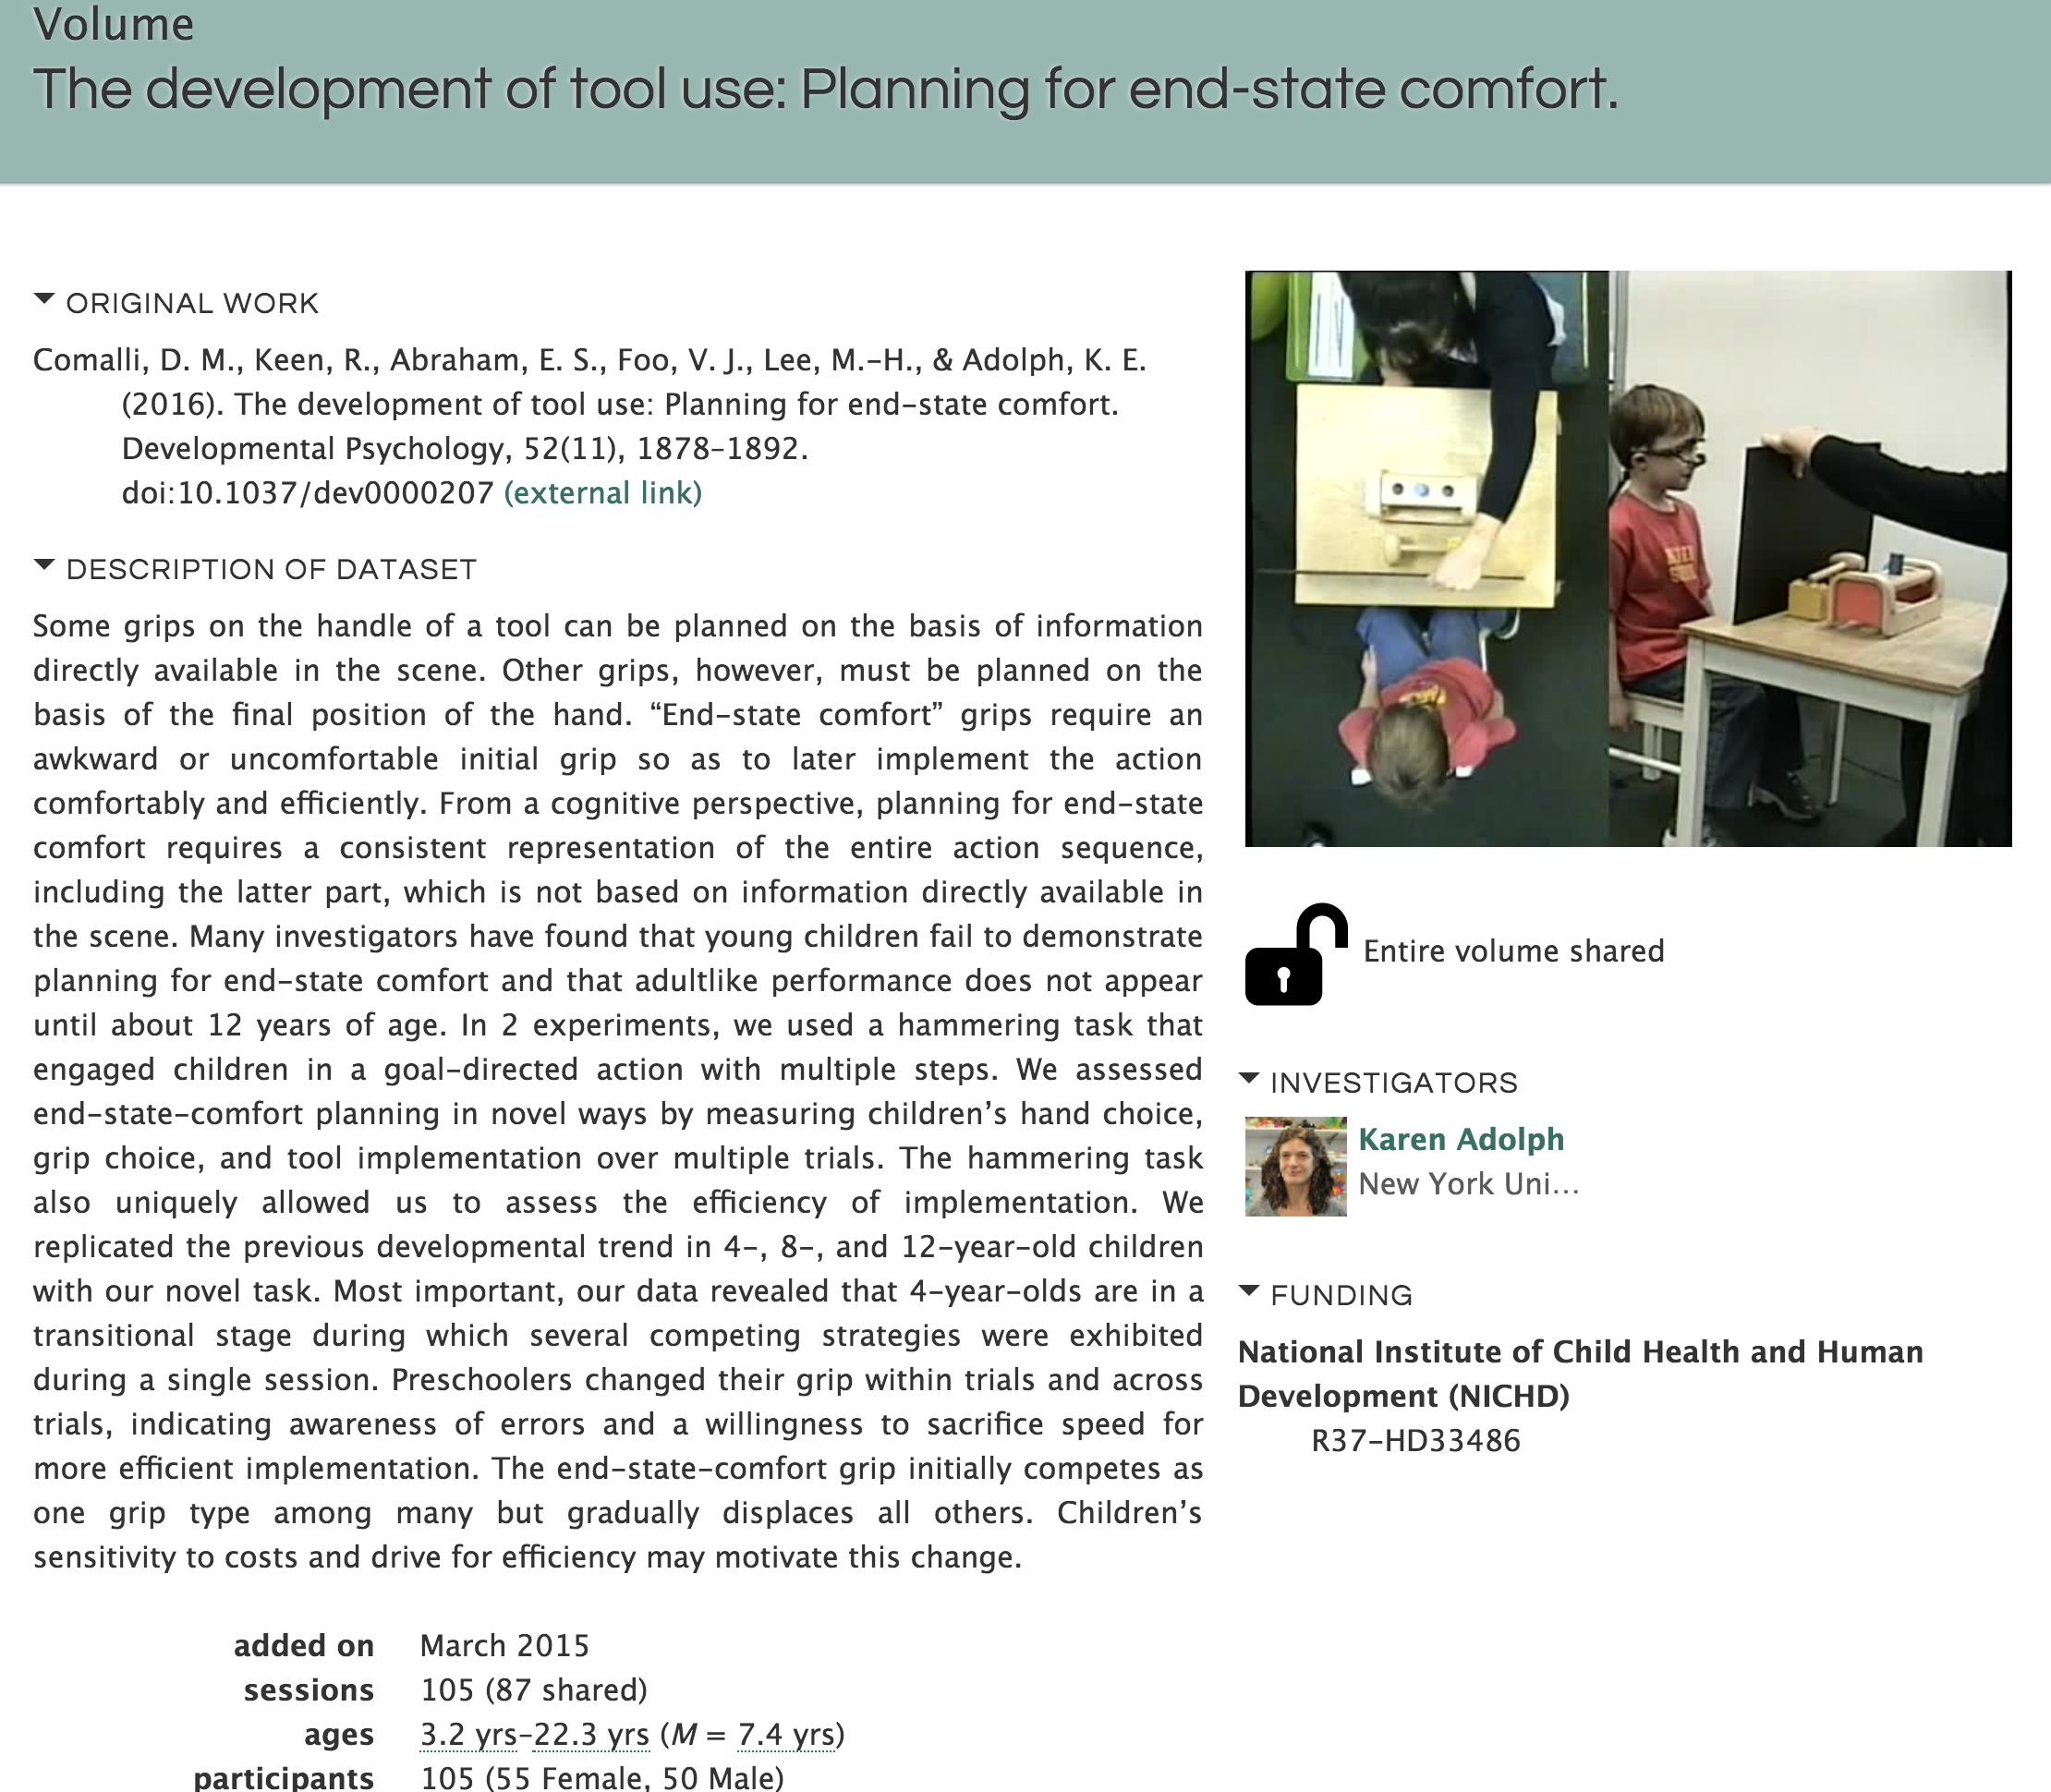
\includegraphics[scale=0.32,valign=t]{img/volume114.png}
\end{center}

\begin{multicols}{3} 
    \tiny
    \par Tamis-LeMonda, C. (2013). Language, cognitive, and socio-emotional skills from 9 months until their transition to first grade in U.S. children from African-American, Dominican, Mexican, and Chinese backgrounds. Databrary. Retrieved September 25, 2018 from http://doi.org/10.17910/B7CC74.
    \columnbreak
    \par Bergelson, E. (2017). SEEDLingS 6 Month. Databrary. Retrieved September 25, 2018 from http://doi.org/10.17910/B7.330.
    \columnbreak
    \par Adolph, K. (2015). The development of tool use: Planning for end-state comfort. Databrary. Retrieved September 25, 2018 from http://doi.org/10.17910/B7.114. 
\end{multicols} 
}
%%%%%%%%%%%%%%%%%%%%%%%%%%%%%%%%%%%%%%%%%%%%%%%%%%%%%%%%%%%%%%%%%%%%%%%%%%%%%%
\headerbox{Video as Documentation}{name=videoDoc,column=1,span=3,row=1, below=videoData}
%%%%%%%%%%%%%%%%%%%%%%%%%%%%%%%%%%%%%%%%%%%%%%%%%%%%%%%%%%%%%%%%%%%%%%%%%%%%%%
%3 horizontally: volume 86, volume 44, PLAY wiki include a video such as initial call
{
\begin{center}
    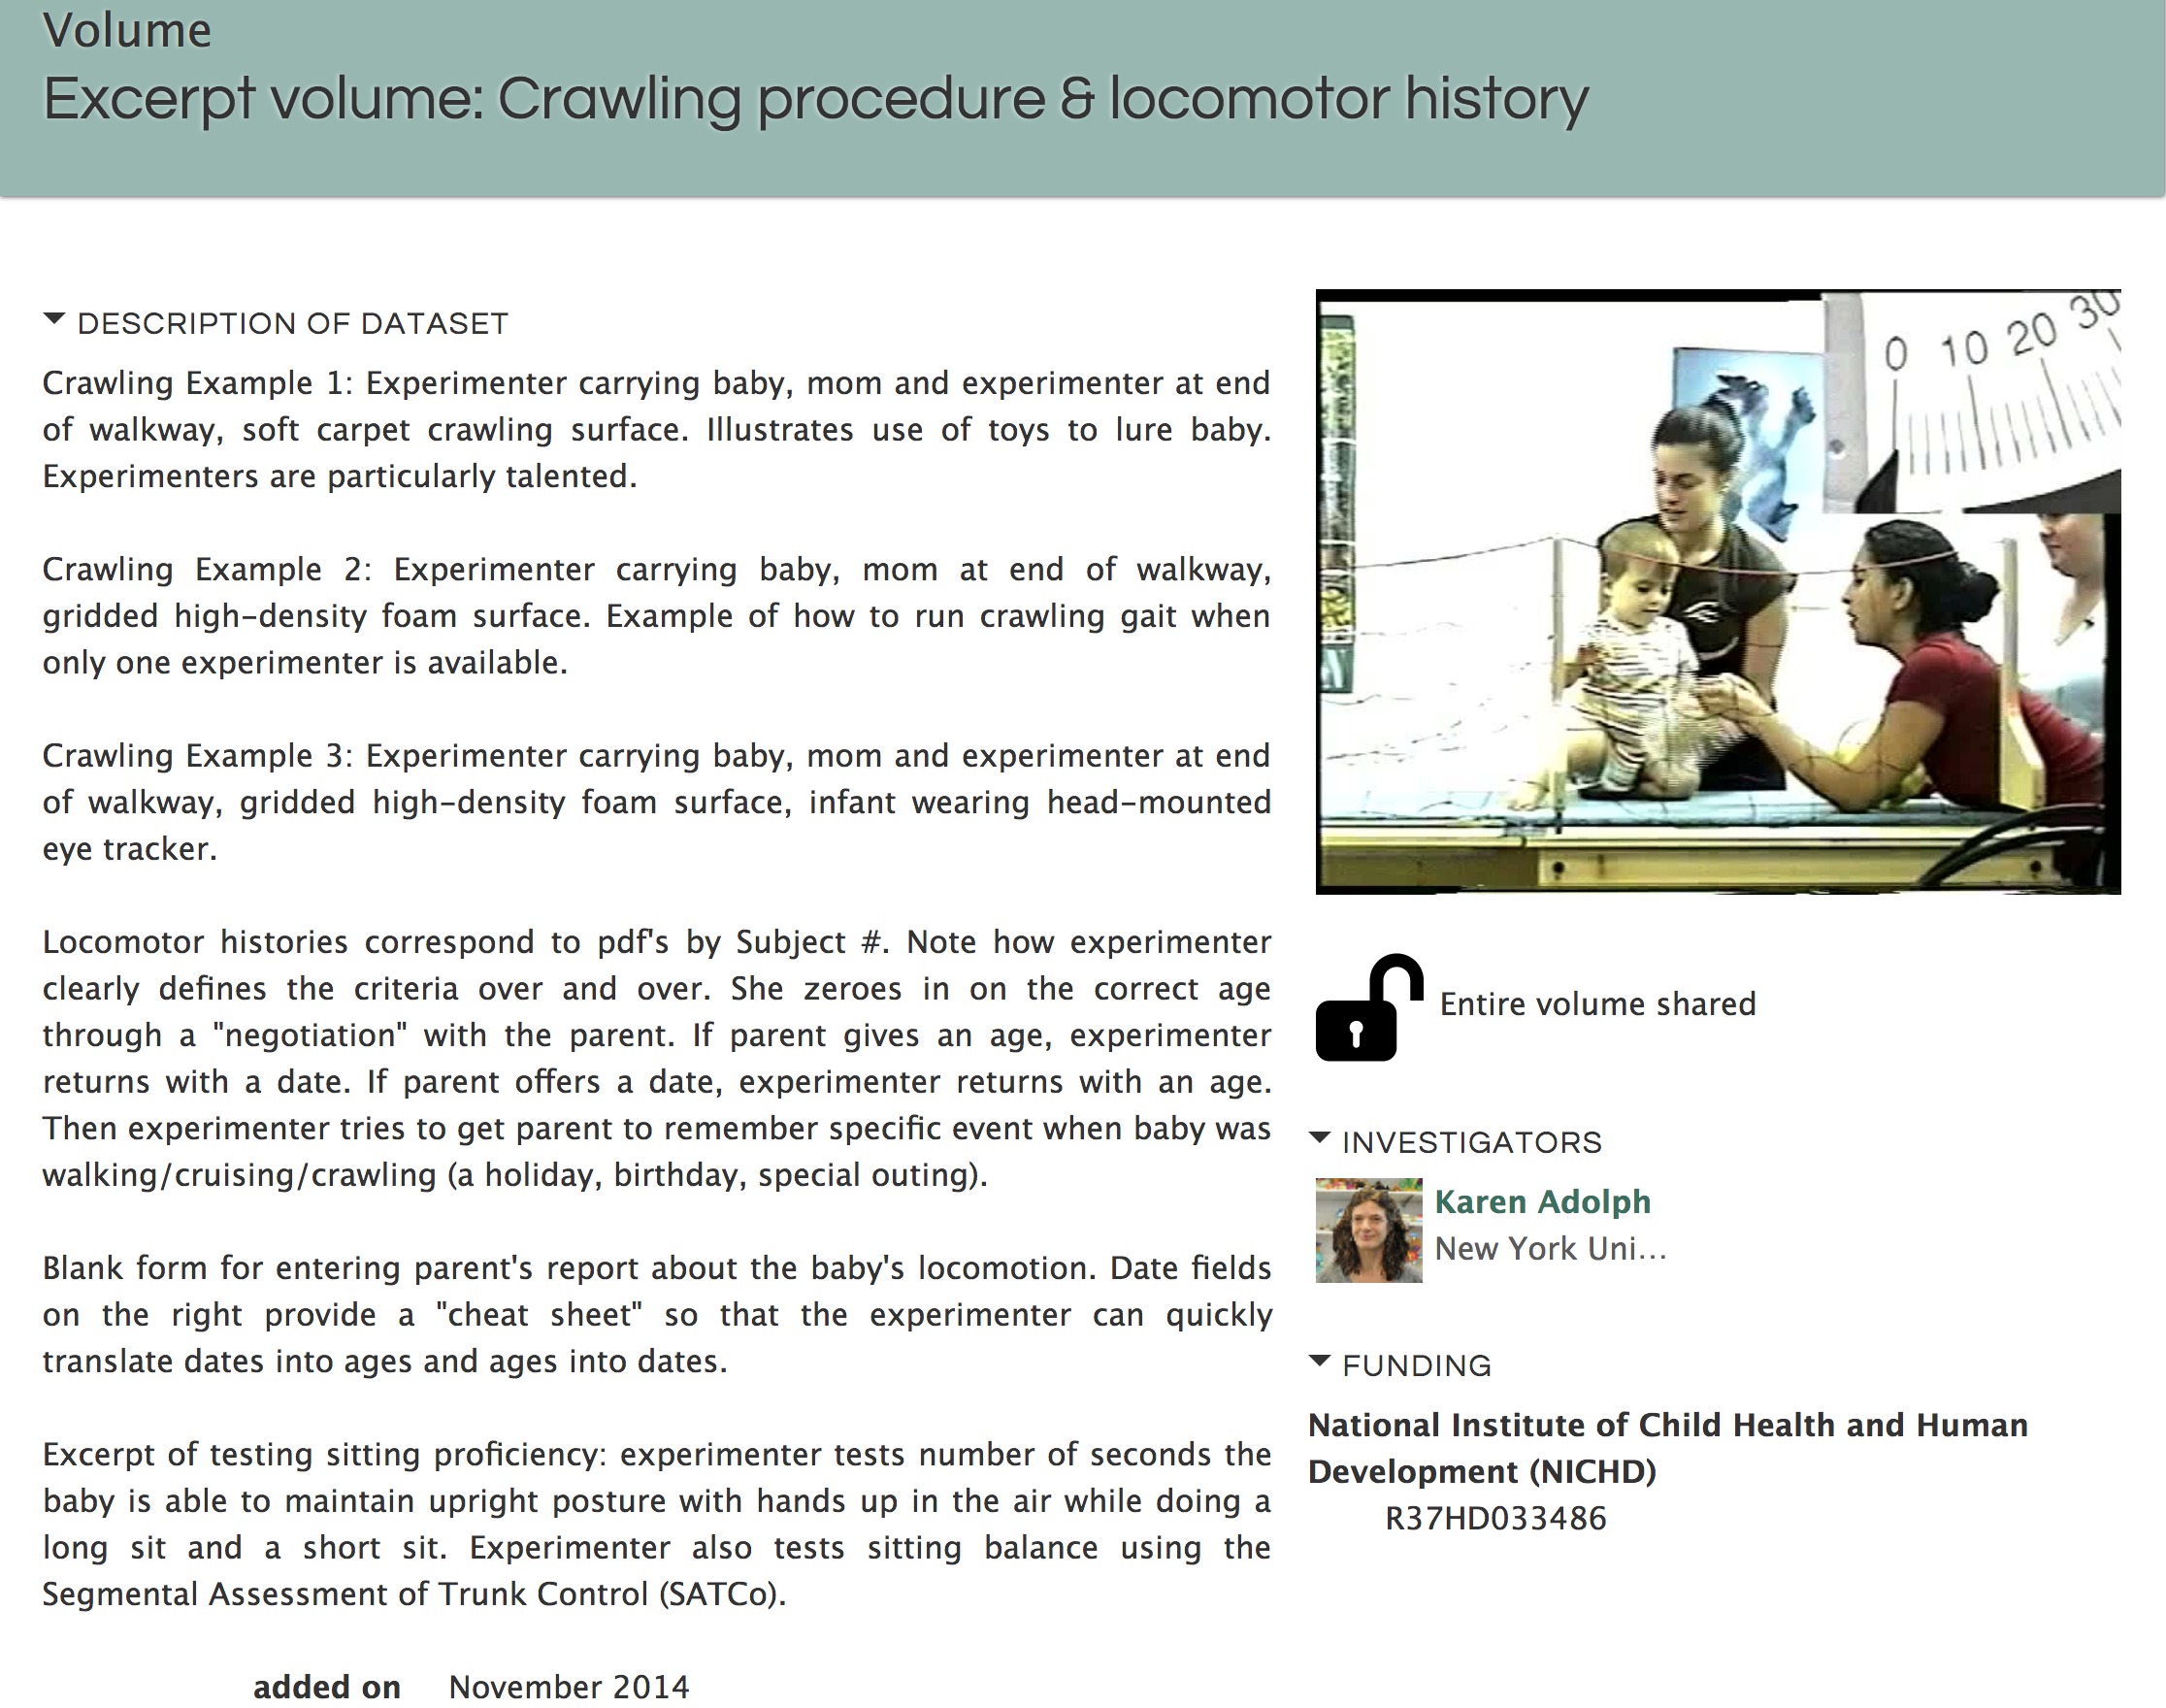
\includegraphics[scale=0.32,valign=t]{img/volume86.png}
    \hfill
    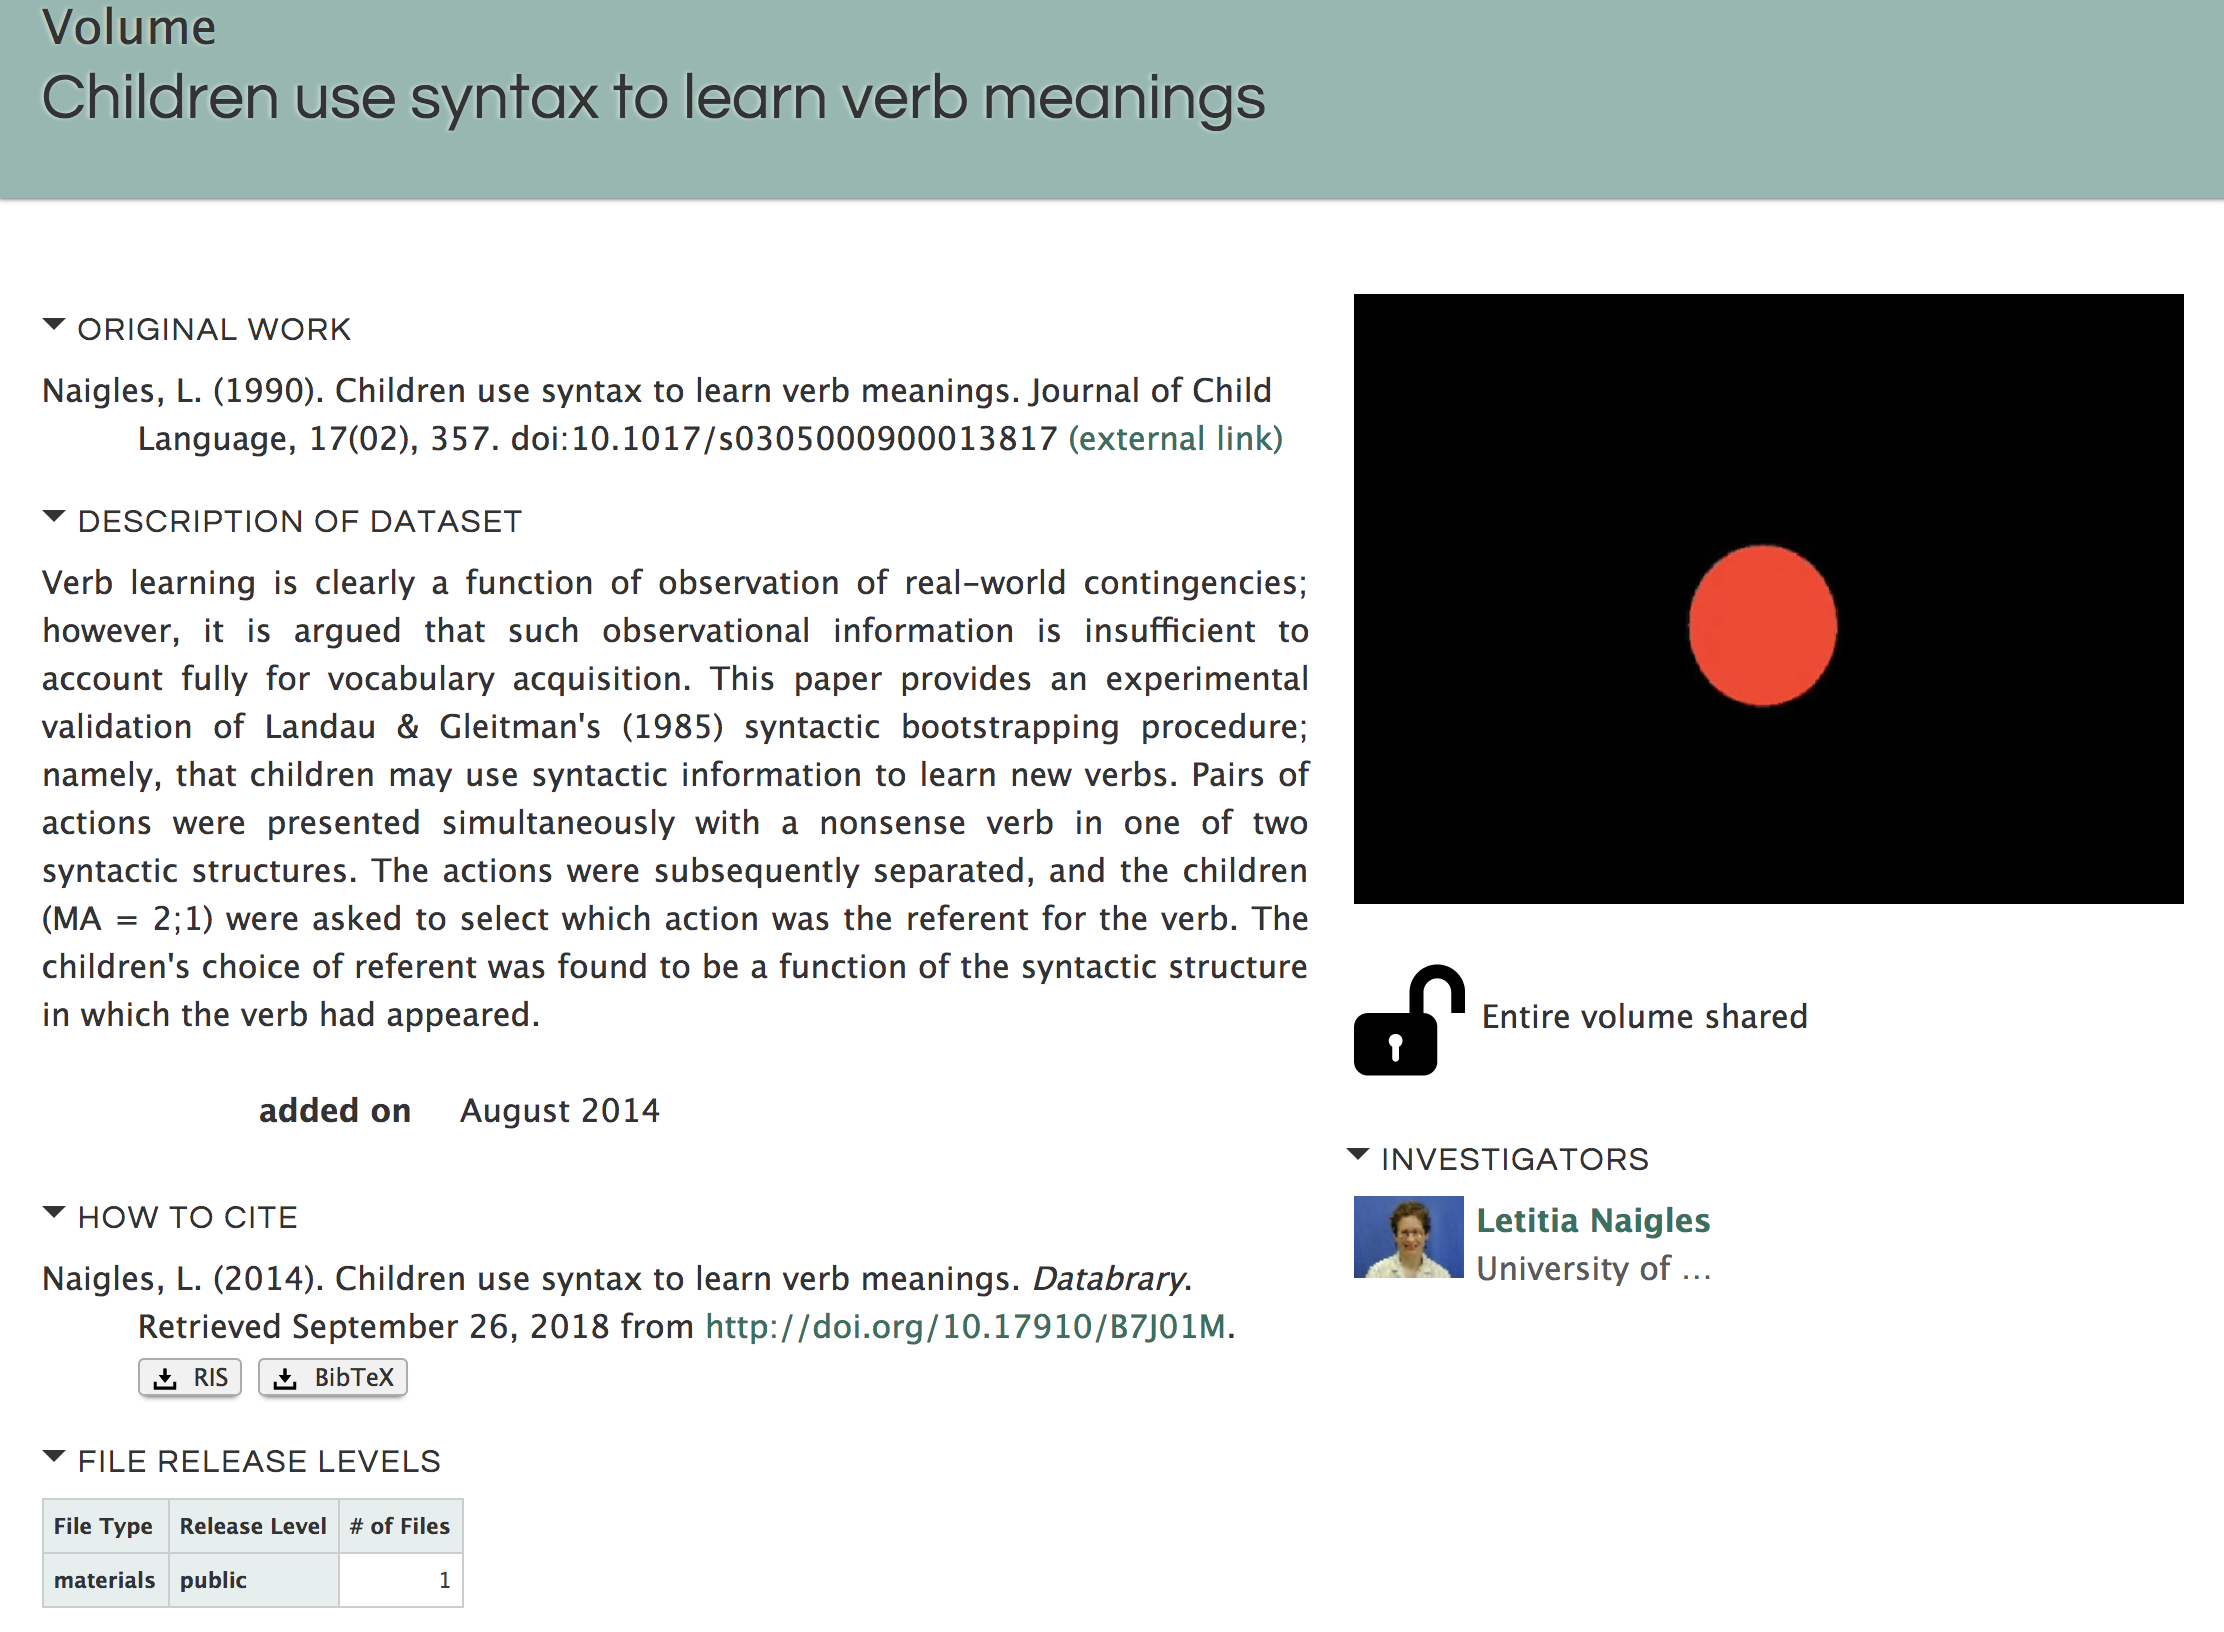
\includegraphics[scale=0.32,valign=t]{img/volume44.png}
    \hfill
    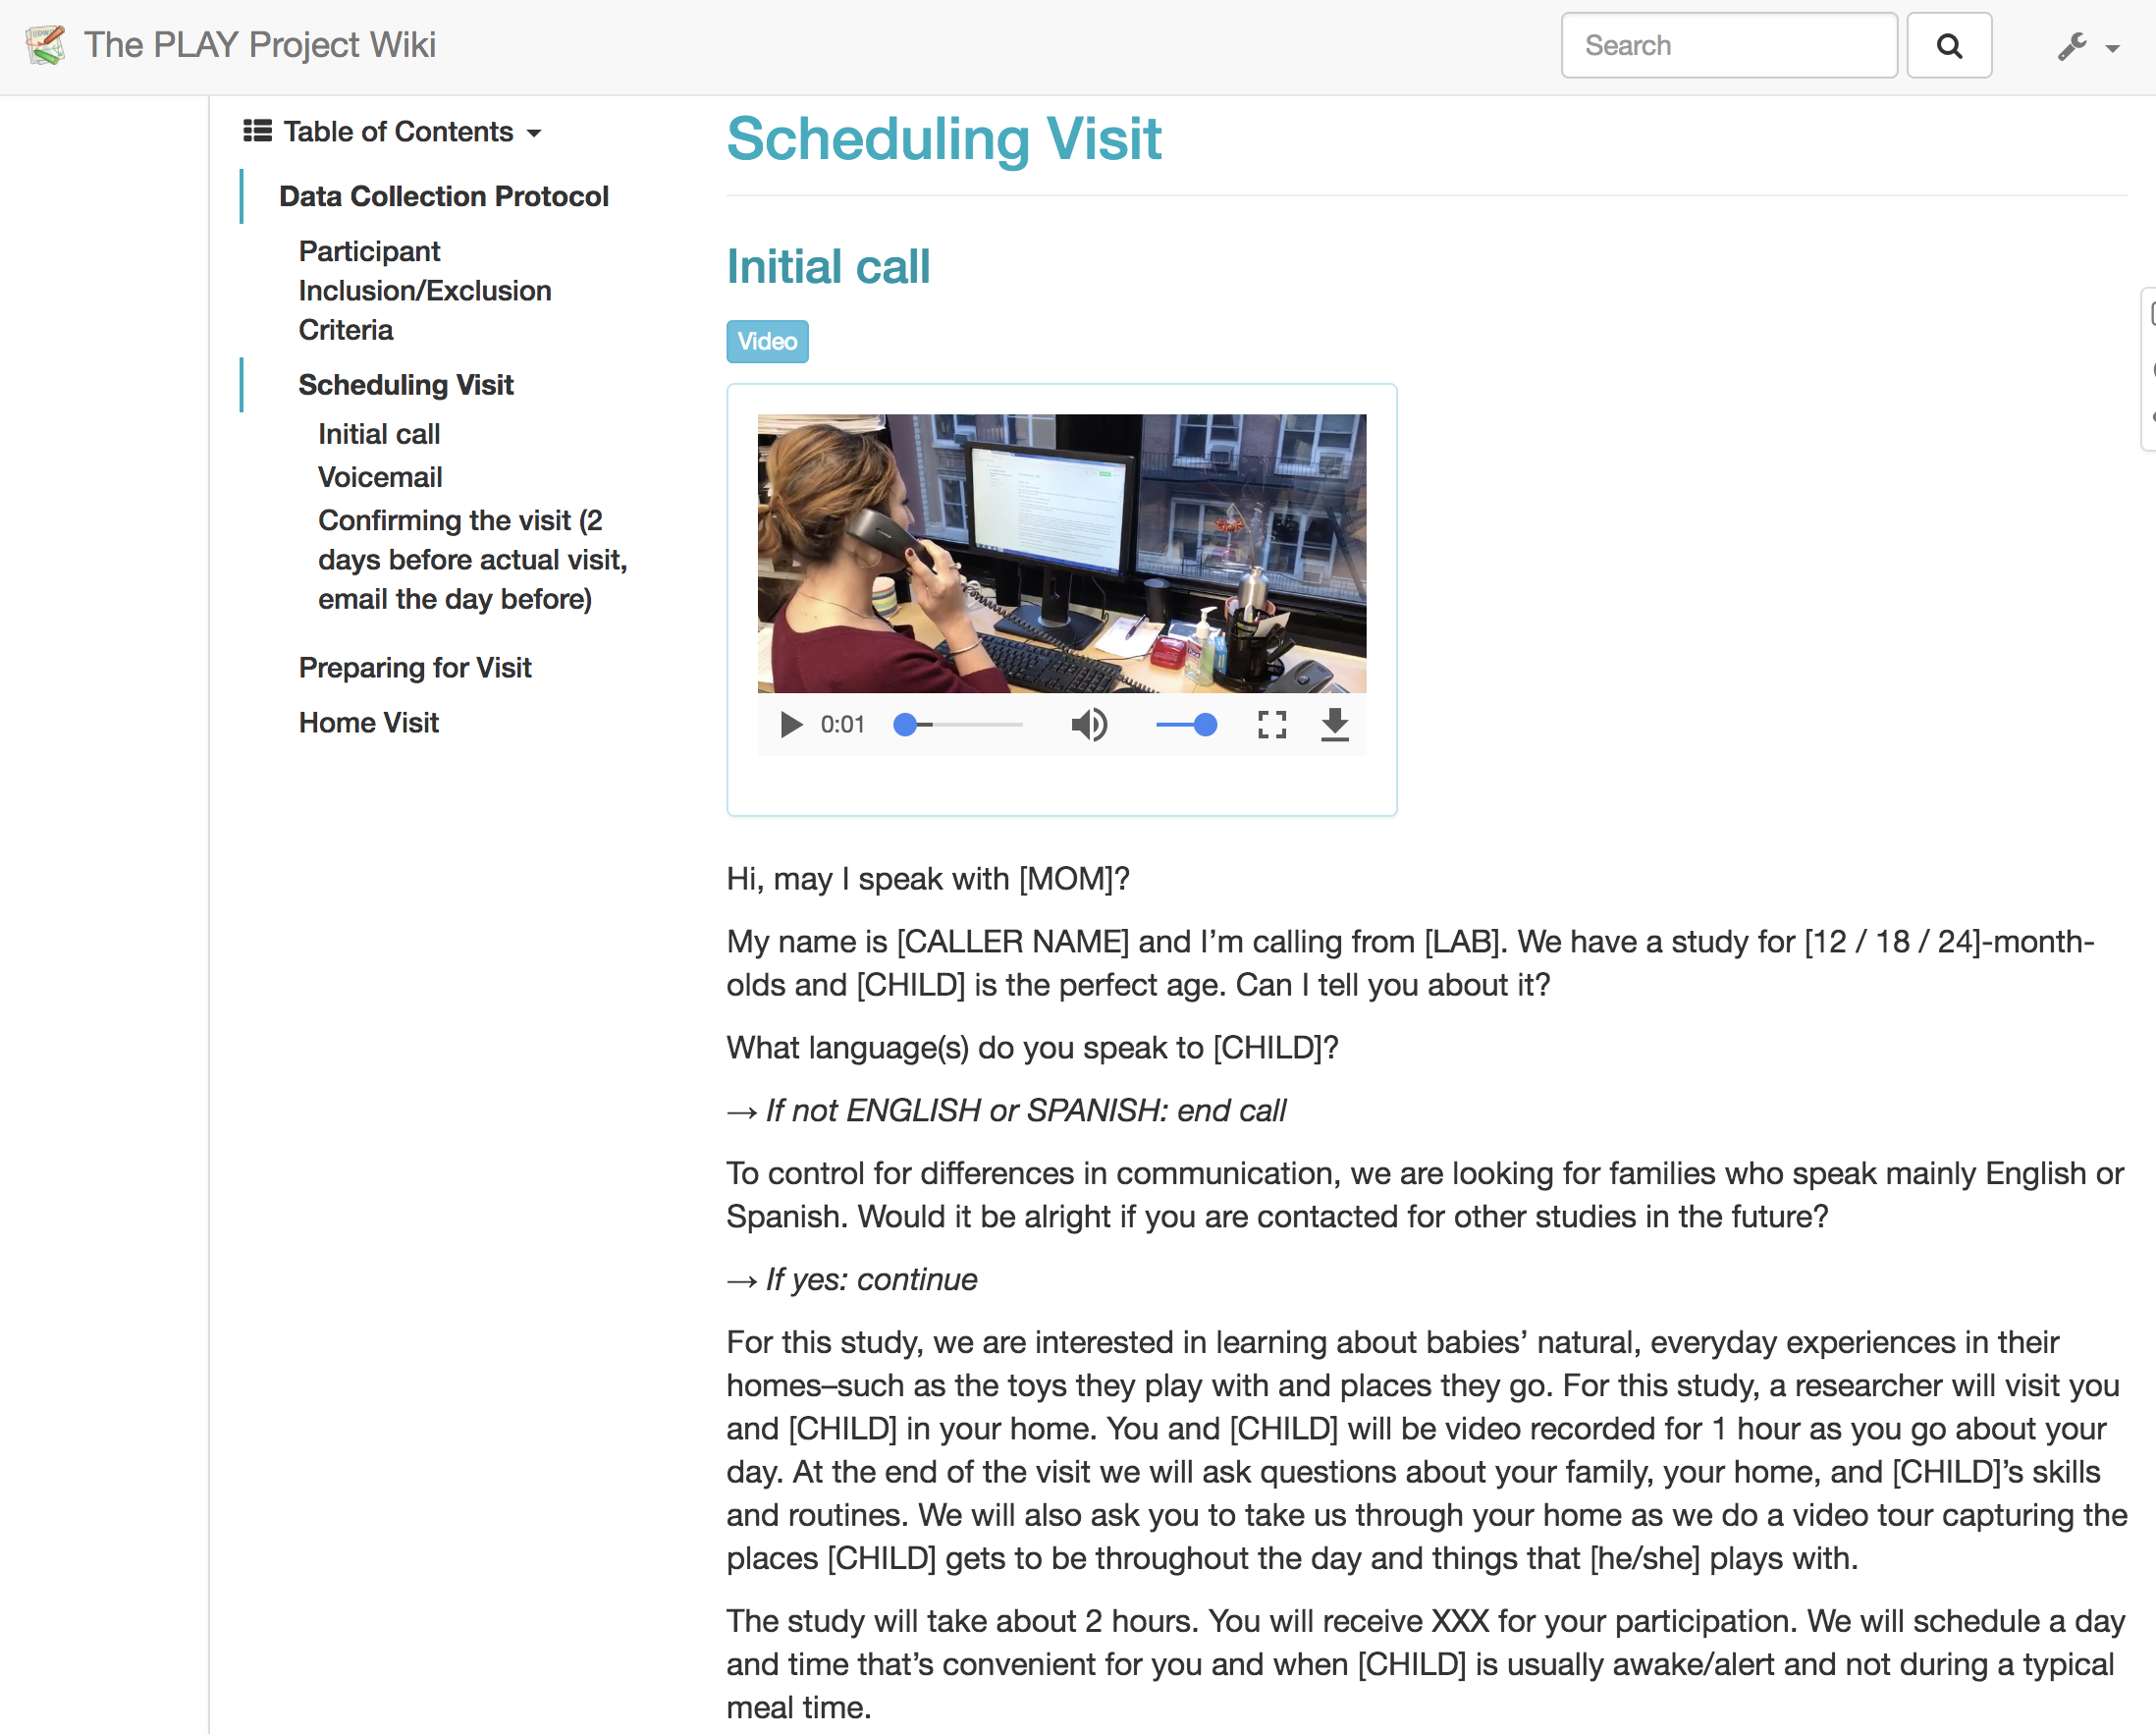
\includegraphics[scale=0.32,valign=t]{img/PLAY-Wiki.png}
\end{center}

\begin{multicols}{3} 
    \tiny
    \par Adolph, K. (2014). Excerpt volume: Crawling procedure \& locomotor history. Databrary. Retrieved September 25, 2018 from http://doi.org/10.17910/B75K5K.
    \columnbreak
    \par Naigles, L. (2014). Children use syntax to learn verb meanings. Databrary. Retrieved September 25, 2018 from http://doi.org/10.17910/B7J01M.
    \columnbreak
    \par The PLAY Project Wiki. Retrieved from https://dev1.ed-projects.nyu.edu/wikis/docuwiki/doku.php.
\end{multicols}
}
%%%%%%%%%%%%%%%%%%%%%%%%%%%%%%%%%%%%%%%%%%%%%%%%%%%%%%%%%%%%%%%%%%%%%%%%%%%%%%
\headerbox{Policies for Sharing}{name=policies,column=0,span=1,below=whatDatabrary, above=bottom}
%%%%%%%%%%%%%%%%%%%%%%%%%%%%%%%%%%%%%%%%%%%%%%%%%%%%%%%%%%%%%%%%%%%%%%%%%%%%%%
{
Databrary enables the open sharing of identifiable video and audio data while protecting confidentiality by:
\begin{itemize}
    \item Securing permission to share from participants and reporting that permission consistently and clearly
    \vspace{-.5em}
    \item Limiting access to authorized individuals via institutional agreements
\end{itemize}    

\begin{center}
  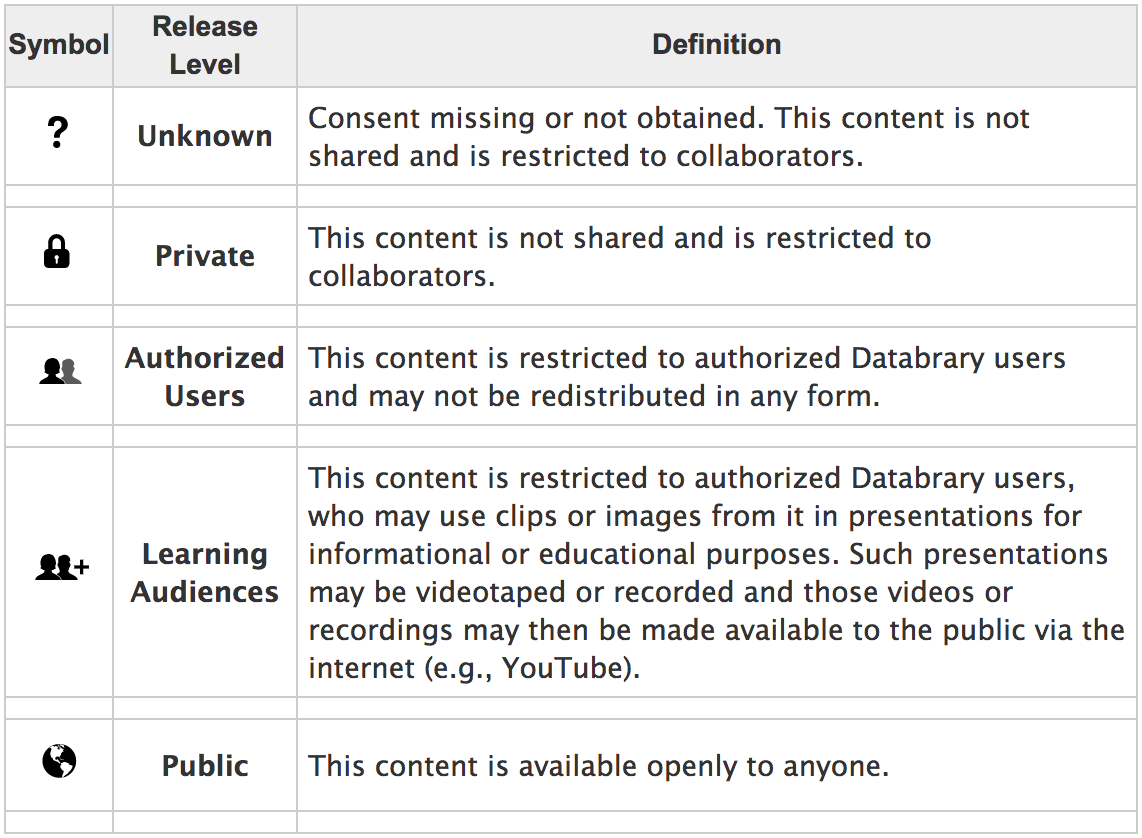
\includegraphics[scale=0.52,valign=t]{img/DatabraryReleaseLevels.png}
\end{center}
}
%%%%%%%%%%%%%%%%%%%%%%%%%%%%%%%%%%%%%%%%%%%%%%%%%%%%%%%%%%%%%%%%%%%%%%%%%%%%%%
\headerbox{Data Sharing Around the World}{name=sharing,column=1,span=2, below=videoDoc, above=bottom}
%%%%%%%%%%%%%%%%%%%%%%%%%%%%%%%%%%%%%%%%%%%%%%%%%%%%%%%%%%%%%%%%%%%%%%%%%%%%%%
{
\begin{center}
    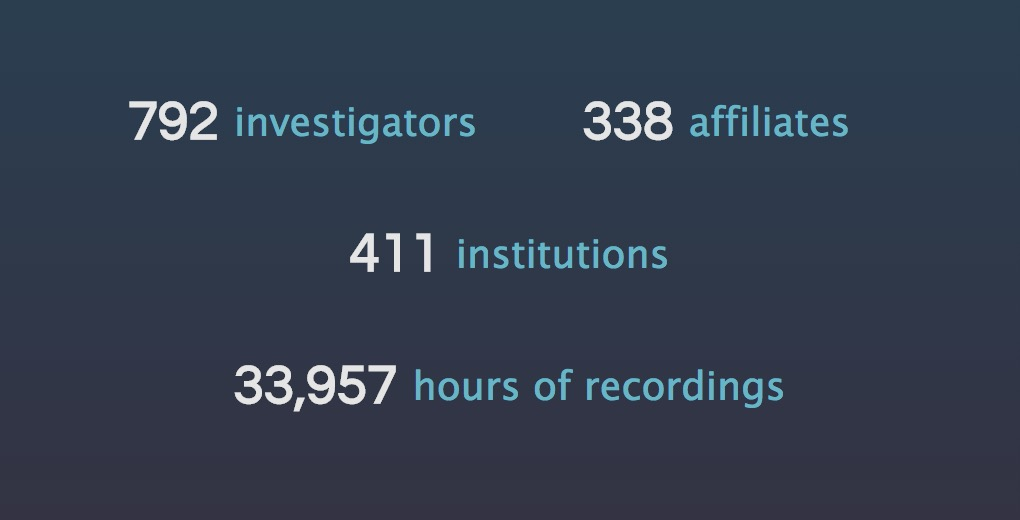
\includegraphics[scale=0.30]{img/databrary-stats.jpg}
    \hfill
    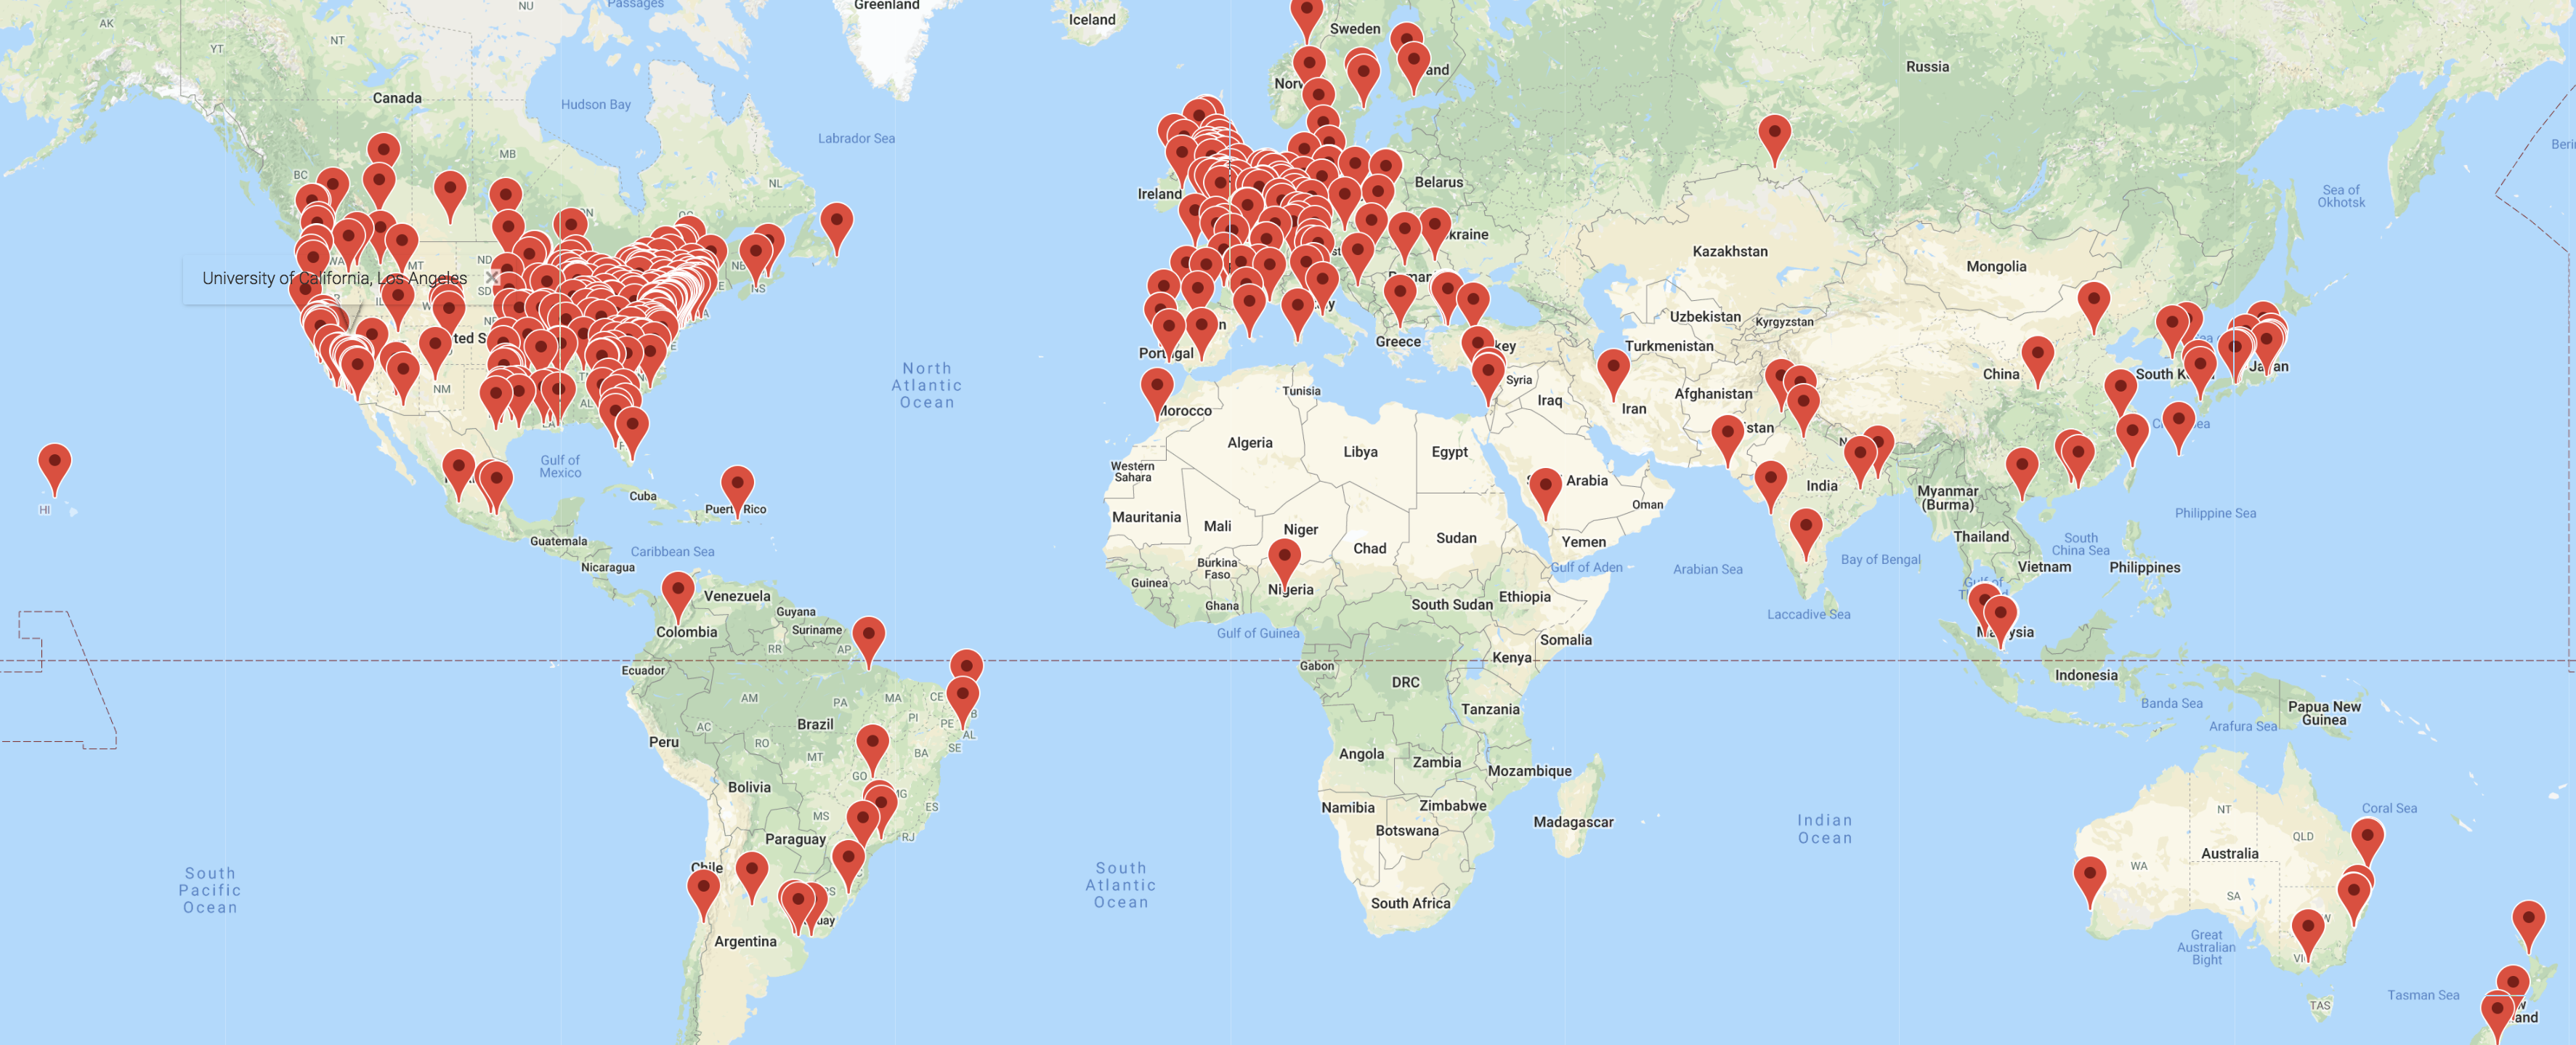
\includegraphics[scale=0.22]{img/databrary-map.png}
\end{center}
}
%%%%%%%%%%%%%%%%%%%%%%%%%%%%%%%%%%%%%%%%%%%%%%%%%%%%%%%%%%%%%%%%%%%%%%%%%%%%%%
\headerbox{Acknowledgements}{name=thanks,column=3,span=1, below=videoDoc, above=bottom}
%%%%%%%%%%%%%%%%%%%%%%%%%%%%%%%%%%%%%%%%%%%%%%%%%%%%%%%%%%%%%%%%%%%%%%%%%%%%%%
{
\begin{center}
    
\includegraphics[scale=0.5,valign=t]{img/nyu.png}
    \hspace{4em}
    
\includegraphics[scale=0.5,valign=t]{img/psu.png}
    
\includegraphics[scale=0.5,valign=t]{img/nichd.png}
    \hspace{4em}
    
\includegraphics[scale=0.5,valign=t]{img/nsf.png}
    
\includegraphics[scale=0.5,valign=t]{img/sloan.png}
    \hspace{4em}
    
\includegraphics[scale=0.5,valign=t]{img/lego.png}
    
\includegraphics[scale=0.5,valign=t]{img/srcd.png}
\end{center}   

} 

\end{poster}%
%
\end{document}
